\clearpage
\Question{Binary Search}

%% Modify the new lines the code for search so that the line numbers
%% differ from semester to semester

Consider the \lstinline'search' function we analyzed in the last
written assignment. This function returned the index of the first occurrence
of $x$ in the array $A$, or -1 if $x$ is not found.
Now let's fill in the loop body with code that implements the binary
search algorithm (on a sorted array, of course).

%\lstinputlisting[numbers=left]{\code/search.c0}
\enlargethispage{5ex}
\begin{lstlisting}[numbers=left]
int search(int x, int[] A, int n)
//@requires 0 <= n && n <= \length(A);[*\label{l:pre1}*]
//@requires is_sorted(A, 0, n);[*\label{l:pre2}*]
/*@ensures (\result == -1 && !is_in(x, A, 0, n))[*\label{l:post1-ab}*]
        || (0 <= \result && \result < n[*\label{l:post2-ab}*]
            && A[\result] == x[*\label{l:post2-c}*]
            && (\result == 0 ||
                A[\result-1] < x)); @*/[*\label{l:post2-d}*]
{
  int lo = 0;
  int hi = n;

  while (lo < hi)[*\label{l:loop-guard}*]
  //@loop_invariant 0 <= lo;[*\label{l:LI1}*]
  //@loop_invariant lo <= hi;[*\label{l:LI2}*]
  //@loop_invariant hi <= n;[*\label{l:LI3}*]
  //@loop_invariant gt_seg(x, A, 0, lo);[*\label{l:LI4}*]
  //@loop_invariant le_seg(x, A, hi, n);[*\label{l:LI5}*]
  {
    if (A[lo] == x)[*\label{l:if1}*]
      return lo;[*\label{l:return1}*]
    int mid = lo + (hi-lo)/2;
    if (A[mid] < x)
      lo = mid+1;
    else { /*@assert(A[mid] >= x); @*/
      hi = mid;
    }
  }
  //@assert lo == hi;
  if (lo != n && A[lo] == x) return lo;
  return -1;
}
\end{lstlisting}
Here is a graphical representation of the loop invariants of this
function:\vspace{-2.5ex}
\begin{center}
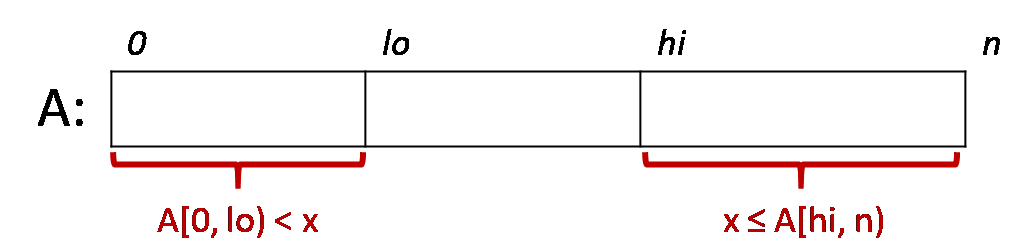
\includegraphics[width=0.75\linewidth]{\img/binsearch-first.png}
\end{center}



\newpage
\begin{parts}
\part[1\half]\TAGS{correctness}
Prove that, in the case that the code returns on line~\ref{l:return1},
the postcondition on lines \ref{l:post1-ab}--\ref{l:post2-d} always
evaluates to true.  We've given the starting facts you'll use in this
proof.  Justify your answers using line numbers or previous steps.

\begin{framed}
When we start an arbitrary iteration of the loop, we know the following:

\begin{enumerate}[{\footnotesize\em A.}]
  \itemindent=-1.3em
  \labelsep=1.2em
\item%
  \lstinline'0 <= n && n <= \length(A)'
  \hfill by line~\ref{l:pre1} (precondition 1)
  %\lstinline'A' and \lstinline'n' are never modified by the function)
\item%
  \lstinline'A[0,n)' \textsc{sorted}
  \hfill by line~\ref{l:pre2} (precondition 2)
  %\lstinline'A' and \lstinline'n' are never modified by the function and
  %\lstinline'A' is not written to anywhere)
\item%
  \lstinline'lo < hi'
  \hfill by line~\ref{l:loop-guard} (loop guard)
\item%
  \lstinline'0 <= lo && lo <= hi && hi <= n'
  \hfill by lines~\ref{l:LI1}--\ref{l:LI3} (loop invariants 1--3)
\item%
  \lstinline'lo == 0 || x > A[lo-1]'
  \hfill by line~\ref{l:LI4} (loop invariant 4)
\item%
  \lstinline'hi == n || x <= A[hi]'
  \hfill by line~\ref{l:LI5} (loop invariant 5)

\ifprintanswers{\color{\answerColor}
\item%
  \lstinline'0 <= \result' by line~\ref{l:if1} %
  (\lstinline'\result == lo') and line~\ref{l:LI1} %
  (\lstinline'0 <= lo').
\item%
  \lstinline'\result < n' by line~\ref{l:if1} %
  (\lstinline'\result == lo'), line~\ref{l:loop-guard} %
  (\lstinline'lo < hi'), and line~\ref{l:LI3} (\lstinline'hi <= n').
\item%
  \lstinline'A[\result] == x' by line~\ref{l:if1} %
  (\lstinline'\result == lo', \lstinline'A[lo] == x').
\item%
  \lstinline'\result == 0 || A[\result-1] < x' by line~\ref{l:if1} %
  (\lstinline'\result == lo')  and either line~\ref{l:LI4} %
  (\lstinline'gt_seg(x, A, 0, lo)') or as given above
  (\lstinline'lo == 0 || x > A[lo-1]').

}\else~\vspace{14cm}\fi
\end{enumerate}
\end{framed}

\RUBRIC
Part (correctness)
TAGS: correctness

Gradescope rubric:
+0.25pt Identify that 0 <= \result (line IF1 says \result == lo, and line LI1 says 0 <= lo)
+0.25pt Identify that \result < n (line IF1 says \result == lo, line LG says lo < hi, and line LI2 says hi <= n)
+0.5pt Identify that A[\result] == x (line IF1 says \result == lo and A[lo] == x)
+0.5pt Identify that \result == 0 || A[\result-1] < x (line IF1 says \result == lo, line LI4 says either [[ x > A[0..lo) ]], or [[ lo == 0 || x > A[lo-1] ]], which are equivalent statements)

Commentary:
- When entering the rubric, replace the following meta-variables with the corresponding line numbers:
  . IF1 = ``if (A[lo] == x)''
  . LI1 = first loop invariant
  . LI2 = second loop invariant
  . LI4 = fourth loop invariant
  . LG = loop guard

  Because the question statement mentions all line numbers, it's not
  critical that they get all the line numbers just right in their
  proof. What I'm looking for here is that they try to justify all the
  parts of the postcondition with the right givens.

  The important steps, half a point each, are:
  . 0 <= \result by line IF1 (\result == lo) and line LI1 (0 <= lo)
  . \result < n by line IF1 (\result == lo), line LG (lo < hi), and
    line 14 (hi <= n)
  . A[\result] == x by line IF1 (\result == lo, A[lo] == x)
  . \result == 0 || A[\result-1] < x by line IF1 (\result == lo)
    and either line LI4 (gt_seg(x, A, 0, lo)) or as given above
    (lo == 0 || x > A[lo-1])

  The line IF1 (\result == lo) justifications are optional.

  The first _TWO_ parts of the postcondition with _extra_
  justifications should be counted as incorrect unless those
  justifications are relevant to the safety of the postcondition.
ENDRUBRIC


\newpage
\part[1]\TAGS{correctness, search}
Argue that the loop has to terminate. Follow the format for
termination arguments described in class and in prior homework!
\begin{framed}
\ifprintanswers{\color{\answerColor}
  The quantity \lstinline'hi-lo' is always decreasing and can never be
  negative as stated in the loop invariant. Thus, the loop will
  terminate.
}\else~\vspace{1.1in}\fi
\end{framed}

\RUBRIC
Part (termination)
TAGS: correctness, search

Gradescope rubric:
+0.5pt Direction correctly specified and always STRICTLY changes during the loop (hi-lo strictly decreases)
+0.5pt Identification of a bound that's ensured by the loop invariants or loop guard (hi-lo can't become negative because of lines LG or LI).

Commentary:
- When entering the rubric, replace the following meta-variables with the corresponding line numbers:
  . LG = 12 (line of the loop guard)
  . LI = 14 (line of the 2nd loop invariant)

The quantity "hi - lo" is always decreasing and can never be
negative as stated in the loop invariant. Thus, the loop will terminate.
. 1/2 point for direction (the quantity hi-lo decreases)
. 1/2 point for bound ("and never becomes negative" is okay, "and
  reaches zero which stops the loop" is okay - doesn't need to cite
  loop invariant specifically)
. Other answers possible, but I don't expect to see other correct
  answers. No partial credit for using "hi" or "lo" as the
  quantity.

Note: It's time to retire this part -- asking just to combine established facts
ENDRUBRIC



\part[2\half]\TAGS{correctness, divide-and-conquer, loop-invariant, safety, search}
On the next page, modify the search function above so that it uses the
binary search algorithm to return the index of the \emph{last}
occurrence of $x$ in array $A$ (as opposed to the first occurrence) or
-1 if $x$ is not found. Think carefully about the contracts to make
sure that your array accesses are safe and that the function is
logically correct.  Here's a picture of the loop invariants you are
aiming for, and that you should express in C0 on
lines~\ref{l:binsearch-last-LI4} and~\ref{l:binsearch-last-LI5}.
Study them carefully.
\begin{center}
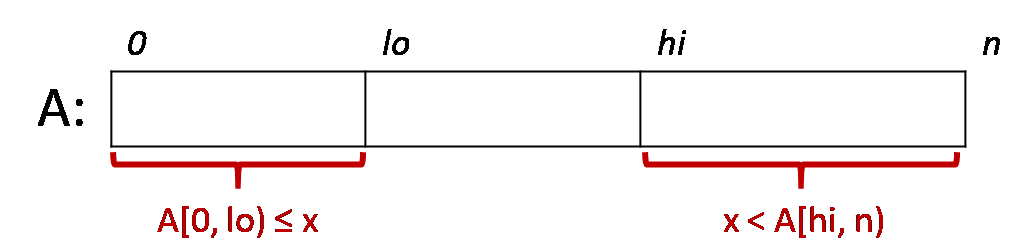
\includegraphics[width=0.75\linewidth]{\img/binsearch-last.png}
\end{center}

There are operationally correct implementations for which it is not
possible to prove that the postconditions are true.  Such
implementations will not get full credit.


\newpage
\begin{lstlisting}[frame=single, numbers=left]
int search(int x, int[] A, int n)
//@requires 0 <= n && n <= \length(A);
//@requires is_sorted(A, 0, n);
/*@ensures (\result == -1 && !is_in(x, A, 0, n))
        || (0 <= \result && \result < n
            && A[\result] == x

            && [*\uanswer{26em}{(\result{} == n-1 || A[\result+1] > x)}*]); @*/
{
  int lo = 0;
  int hi = n;

  while (lo < hi)
  //@loop_invariant 0 <= lo;
  //@loop_invariant lo <= hi;
  //@loop_invariant hi <= n;

  //@loop_invariant [*\uanswer{26em}{ge\_seg(x, A, 0, lo)}*];[*\label{l:binsearch-last-LI4}*]

  //@loop_invariant [*\uanswer{26em}{lt\_seg(x, A, hi, n)}*];[*\label{l:binsearch-last-LI5}*]
  {
    int mid = lo + (hi-lo)/2;

    if ([*\uanswer{25.8em}{A[mid] <= x}*]) lo = mid+1;

    else { /*@assert([*\uanswer{22.2em}{A[mid] > x}*]); @*/
      hi = mid;
    }
  }
  //@assert lo == hi;

  if ([*\uanswer{33.2em}{hi != 0 \&\& A[hi - 1] == x}*]) {

      return [*\uanswer{30.3em}{hi - 1}*];
  }

  return -1;
}

\end{lstlisting}

\RUBRIC
Part (last occurrence)
TAGS: correctness, divide-and-conquer, loop-invariant, safety, search

Gradescope rubric:
+ 0.25 pts L8: postcondition ensures correctness ... in most cases (e.g., A[\result+1] > x)
+ 0.25 pts L8: postcondition is ALSO safe (e.g., \result == n-1 || A[\result+1] > x)
+ 0.5 pt L17,19: ge_seg(x, A, 0, lo), lt_seg(x, A, hi, n)
+ 0 pts -- OR -- Unsafe loop invariant (no points for rest of the question)
+ 0 pts -- OR -- Other loop invariants that bound [lo..hi) (changes grading of the rest of the question)
+ 0 pts -- OR -- Other incorrect loop invariants
+ 0.5 pt L23: A[mid] <= x
+ 0.5 pt L25: A[mid] > x (or is a logical consequence of the negation of line 23, if line 23 is wrong)
+ 0.25 pts L31,33: Conditional is essentially correct (e.g. if (A[hi-1] == x) return hi-1; or if (A[lo-1] == x) return lo-1;)
+ 0.25 pts L31,33: Conditional is ALSO safe (e.g. if (hi != 0 && A[hi - 1] == x) return hi - 1; or if (lo != 0 && A[lo-1] == x) return lo - 1;)

Commentary:
Separated into five parts, currently the only partial
credit is for simple safety violations

. On Line 8, x and A[\result] are interchangable
. Line 8, 1 point:     (\result == n-1 || A[\result+1] > x)
. Line 8, 1 point:     (\result == n-1 || A[\result+1] != x)
. Line 8, 1 point:     lt_seg(x, A, \result+1, n)
. Line 8, 1 point:     !is_in(x, A, \result+1, n)
. Line 8, 1/2 point:   (A[\result+1] > x)
. Line 8, 1/2 point:   (A[\result+1] != x)
. Line 8, 1/2 point:   (A[\result+1] > x || \result == n-1)
. Line 8, 1/2 point:   (A[\result+1] != x || \result == n-1)

SIMPLEST SOLUTION:
. Lines 17,19, 1 point: ge_seg(x, A, 0, lo), lt_seg(x, A, hi, n)
. Lines 17,19, ANYTHING ELSE PUT ASIDE FOR SECONDARY RUBRIC
        We want to deal with other loop invariants carefully and
        systematically, because the correct answers for lines 31,33
        are dependent on the loop invariant.

. Line 23, 1 point: A[mid] <= x

. Line 25, 1 point: A[mid] > x (or any non-trivial thing that it's
                                correct to conclude from the previous
                                conditionals as the student wrote them)

. Line 31,33, 1 point:   if(hi != 0 && A[hi-1] == x) return hi-1
. Line 31,33, 1 point:   if(lo != 0 && A[lo-1] == x) return lo-1
. Line 31,33, 1/2 point: if(A[hi-1] == x) return hi-1
. Line 31,33, 1/2 point: if(A[lo-1] == x) return lo-1

MORE COMPLEX SOLUTION:
. Lines 17,19, 1 point: ge_seg(x, A, 0, lo), le_seg(x, A, hi, n)
. Line 23, 1 point: mid+1 < n && A[mid+1] <= x
. Line 25, 1 point: mid+1 >= n || A[mid+1] > x
. Line 31,33, 1 point:   if(lo != n && A[lo] == x) return lo  [or same with hi]


One solution is in file code/search-sol.c0

Note:
Alternate 2nd version of (c):
  - return last occurrence of x
  - return first occurrence of x
ENDRUBRIC

\end{parts}
